\documentclass{supervision}
\usepackage{course}

\begin{document}

\begin{questions}
  %%%%%%%%%%%%%%%%%%%%%%%%%%%%%%%%%%%%%%%%%%%%%%%
  \section*{Topic 01 - Introduction / Foundation}
  %%%%%%%%%%%%%%%%%%%%%%%%%%%%%%%%%%%%%%%%%%%%%%%
  \question \textit{Concepts in (computer) networking.}
    Consider a communication network consisting of a room full of people,
    where one or more people are exchanging thoughts with one or more others
    by talking.

    \begin{parts}
      \part For each of the abstract terms node, channel, entity, layer,
        transmission (the act thereof), coding, addressing and multiplexing,
        identify one or more corresponding concrete components or activities
        within the system. If the correspondence is not exact, give the
        closest approximation you can, and explain why it is not exact. [If
        you're unfamiliar with any of the abstract terms, you may need to
        look ahead in the lecture notes, or in one of the course texts.]

      \part Compare and contrast the network with a \textit{shared-media
        wireless ethernet} and a \textit{single ethernet} link, for the
        following channel criteria:

        \begin{itemize}
          \item{physical medium}
          \item{total capacity}
          \item{maximum user-to-user capacity}
          \item{medium access control}
          \item{geographical area}
          \item{failure modes}
        \end{itemize}

      \part Suggest one way in which \textit{administration} (or
        “management”) of a room-full-of-people network may be performed.
        State whether it is distributed, centralised or a mixture of the
        two. [Hint: consider the example of a private party.]
    \end{parts}

  \question{Multiplexing basics}
    \begin{parts}
      \part Give an example of multiplexing in a real system. Using your
        example, explain the relationship between multiplexing and coding.
        Explain your example’s \textit{policy} (concurrency-control) on
        access to the lower-layer channel, and how this is agreed.

      \part Explain the similarity and distinction between \textit{frequency
        division multiplexing} and \textit{wave division multiplexing},
        giving an example of each.

      \part What kind of traffic is suited to \textit{synchronous
        time-division multiplexing}? Define the term \textit{circuit}. Give
        an example of a \textit{circuit} which is \textit{not} implemented
        using time-division multiplexing.

      \part Give three ways in which asynchronous time-division multiplexing
        is more complex than synchronous time-division multiplexing. In what
        circumstances does asynchronous TDM make more efficient use of the
        lower-layer channel than synchronous TDM?

      \part Explain why contention policies are inherently more complex on a
        shared media link than a point-to-point link using asynchronous TDM.
        Give an example of each.

      \part Ethernet is an asynchronous TDM system with a random-access
        contention policy. With reference to collision detection, give one
        reason why shared media Ethernets have a maximum length, and suggest
        how this might be calculated from the bitrate of the link and the
        minimum packet length. Give an example of a link which might use
        asynchronous TDM but where collision detection is not feasible.

      \part Using the example of a two-way radio conversation, explain token
        loss and token duplication in token-based asynchronous TDM.

      \part Explain how slotted systems for asynchronous TDM are different
        from synchronous TDM. In what case are the two equivalent?

      \part The telephone network is an example of a reservation system.
        Explain what is happening when a caller dials a telephone number.
        Give two reasons why the delay between dialing a number and being
        connected (i.e. hearing the remote ringer) is variable.
    \end{parts}

  \question \textit{Supervision discussion questions}
    \begin{parts}
      \part Give an example of multiplexing at all five (seven?) layers in a
        network stack.

    \end{parts}

  %%%%%%%%%%%%%%%%%%%%%%%%%%%%%%%%%%%%%%%%%%%%%%%
  \section*{Topic 02 - Architecture and Internet}
  %%%%%%%%%%%%%%%%%%%%%%%%%%%%%%%%%%%%%%%%%%%%%%%

  \question \textit{Standards - so many to choose from and Internet Philosophy}
    \begin{parts}
      \part The Internet's standards body, the IETF, has a philosophy which
        was summarised by David Clark, one of the Internet's pioneers as
        follows.

        \begin{quote}
          We reject kings, presidents and voting. We believe in rough
          consensus and running code.
        \end{quote}

        This suggests an approach which is open, dynamic and led by
        implementation. By contrast, other standards bodies such as the ITU
        are closed, slow-moving and led by specification. Using examples,
        discuss ways in which the IETF’s approach has enabled innovation in
        the Internet, and ways in which it has caused problems.

      \part Prior to the Internet, wide-area networks were joined together at
        level of application protocols, using gateways. Explain, as fully as
        you can, why this approach limited application development.

      \part Explain how the design of the Internet protocol, i.e. IP,
        addressed this problem of application development. You should explain
        how the term “hourglass model” describes IP’s approach to network
        layering.

      \part The design of IP makes explicit provision for fragmentation, i.e.
        the ability to split an individual packet into pieces during its
        journey across the network. By considering the hourglass model,
        suggest why this feature is essential.

      \part TCP is a connection-oriented reliable byte-stream protocol designed
        to run over IP, an unreliable conectionless datagram protocol.

        \begin{subparts}
          \subpart Where is the state of a TCP connection held?
          \subpart How does this constrain the set of guarantees offered by a
            TCP connection?
          \subpart In what ways is packet loss essential to TCP's methods of
            modelling the state of the channel (i.e. within the network)?
        \end{subparts}

      \part Comparing (data) delays in packet and circuit-switched networks.
        Compare the time it takes to transfer a file of data under
        circuit-switching and packet-switching. Consider a network consisting
        of $n$ links in a row, each of $B$ bandwidth and latency $L$.

        \begin{description}
          \item[Circuit-switching] At time $t = 0$, the first node sends out a
            circuit reservation packet (of size $R$) which is sent to the
            second node, which then receives the full packet and then forwards
            it to the next node. This is continued at each node, until the
            reservation packet arrives at the last node (after traversing $n$
            links). After this reservation message is processed at the last
            node (the destination), the last node sends back a reservation
            confirmation message (also of size $R$) back to the first hop.
            Because the circuit is established before this confirmation is
            sent, this packet need not be processed at each node; instead, the
            bits flow through the nodes without any delay. Once the
            confirmation message is received at the first node (the source),
            the source immediately starts sending the file (which is of size
            $F$) at the full bandwidth of the link.

            Note that when the file is transferred, the data is not
            stored-and-forwarded at any of the intermediate nodes but is just
            passed through without delay.

            Also, we ignore the teardown message, since it is only sent after
            the file arrives.

            \begin{subparts}
              \subpart Assuming no problems in transmission along the way, at
              what time does the last bit of the file arrive at the last node
              (the destination)?
            \end{subparts}

          \item[Packet-switching] Here the file is broken into $Q$ packets of
            size $D$, each with header size $H$ and payload size $P$. Since
            the entire file must be carried, $Q \times P = F$. At time
            $t = 0$, the source (the first node) sends the first packet, which
            is stored-and-forwarded at each of the subsequent nodes until it
            reaches the destination (the last node). As soon as the source
            finishes sending the first packet, it sends the second packet (at
            full link bandwidth). Note that the source does not wait until the
            first packet arrives at the next node before starting the next
            transmission, it starts sending the next packet as soon as it has
            finished transmitting the previous packet. We assume that a node
            can immediately send a packet out on the next link as soon as the
            last bit has arrived from the previous link (i.e., there is no time
            required to process the packet before sending it on the next link)

            \begin{subparts}
              \SetQuestionNumber{2}
              \subpart Assuming no packet drops or other errors, at what time
                does the last bit of the file arrive at the destination?
            \end{subparts}

            In the following questions, we refer to cases where some quantities
            are big. By that we mean consider the limit where that quantity
            becomes infinitely large or infinitesimally small. Note that some
            quantities are linked (i.e., if the payload $P$ gets smaller, the
            number of packets $Q$ must get larger to keep $Q \times P = F$).
            For each question, the answer could be either: circuit-switched is
            faster, or packet-switched is faster.

            Even if you didn’t get the formulae above completely correct, you
            should understand how these perform relative to each other in the
            limit. Use this as a way to check your answers for the two previous
            questions.

            \begin{subparts}
              \SetQuestionNumber{3}
              \subpart If the file size $F$ is very large, which is faster?
                (Assume that the header size $H$ has not changed.)

              \subpart If the payloads become small (but the header size
                remains constant), which is faster?

              \subpart If the bandwidth $B$ is very large, which is faster?
                And by what ratio (in the limit)?

            \end{subparts}
          \end{description}
        \end{parts}
      \question Internet philosophy
        \begin{parts}
          \part What is the difference between an architectural principle and
            an architectural design (choice)? What other examples can you think
            of?

          \part A NAT stores state about the flows (connections) that pass
            through it.
            \begin{subparts}
              \subpart Why does a NAT break the end-to-end principle?
              \subpart Why might the NAT violation of the end-to-end principle
                not actually matter?
            \end{subparts}
        \end{parts}
      \question \textit{Supervision discussion questions}
        \begin{parts}
          \part What is a defacto standard?
        \end{parts}

      %%%%%%%%%%%%%%%%%%%%%%%%%%%%%%%%%%%%%%%%%%
      \section*{Topic 03 - Data-Link (Physical)}
      %%%%%%%%%%%%%%%%%%%%%%%%%%%%%%%%%%%%%%%%%%

      \question \textit{Shared media multiplexing in local area networks}
        \begin{parts}
          \part Define the term \textit{shared media network}

          \part Explain how Ethernet performs \textit{carrier sense},
            \textit{collision detection}, how it aims to minimise the
            probability of collision on retransmission and how this is adapted
            to handle varying load.

          \part Explain why token ring does not share media at the physical
            level, but is still analyzed as a shared media system.

          \part What is the role of a token monitor in token ring? Why does the
            monitor \textit{not} prevent failure when one of the nodes in the
            ring suffers a hardware failure? Suggest how a token ring system
            might be designed to handle failure of a computer attached to the
            ring.

          \part Explain the meaning of \textit{destination delete} and
            \textit{source delete} as used in ring-based networks.

          \part Explain the difference between conventional token rings and
            \textit{slotted rings}. What are the advantages of a slotted ring?
        \end{parts}

      \question \textit{Multiplexing redux}
        \begin{parts}
          \part Several real-time video streams are to share the same
            lower-layer channel.
            \begin{subparts}
              \subpart Give one example of a lower-layer channel in which the
                flows might be scheduled, and one in which scheduling is not
                possible.

              \subpart A lecturer remarks that “centralised multiplexing”
                offers potential gains in efficiency over non-centralised
                multiplexing. Give two reasons why this can improve efficiency.
                What, in general terms, is the “centralised” facility necessary
                for these gains to be possible?

              \subpart Using an example, describe why specifying a scheduling
                policy in terms of priority may cause problems, even where it
                is safe to use priority within the scheduling mechanism.
                [Hint: consider CPU scheduling in an operating system.]
            \end{subparts}

          \part Code-division multiple access (CDMA) is a code-division
            multiplexing system, used for mobile telephony.
            \begin{subparts}
              \subpart What is a code? What property of codes causes them to be
                “nearly orthogonal” to each other?

              \subpart Two transmitters, A and B, both want to transmit a
                four-bit message at the same time using CDMA. Transmitter A has
                code 10010111 and message 1001. Transmitter B has code 00111101
                and message 0011. Write down the bit sequences transmitted by A
                and B. Write down the bit sequence seen by a receiver, stating
                any assumption you make. Show that the original messages of
                both A and B may be recovered. [Each bit is transmitted as the
                exclusive OR of the code sequence with the bit value.]
            \end{subparts}
        \end{parts}

      \question \textit{Coding, digitisation, error detection and error
        correction}
        \begin{parts}
          \part Give, with examples, three advantages of digitising audio, and
            three corresponding disadvantages. (Compare with storing and
            processing it exclusively on analogue media and equipment.)

          \part Explain quantisation and sampling of analogue signals, and the
            distinction between these. State an upper bound for the
            signal-to-noise ratio of a signal quantised at $b$ bits resolution,
            assuming the analogue original to be noiseless and the quantisation
            process completely accurate.

          \part Outline encode and decode procedures for a simple ($m$,$k$)
            block code. Show that the minimum distance of any simple checksum
            code is always $2$.
        \end{parts}

      \question \textit{CRCs}
        \begin{parts}
          \part Explain, giving an example, how to write a binary message (i.e.
            a sequence of binary digits) as a polynomial.

          \part Outline send and receive procedures for CRC-based message
            coding and error detection. What information must be agreed in
            advance by the sender and reciever?

          \part Draw a shift register which will compute the remainder on
            division of an input polynomial by the CRC-8 polynomial
            $x^8 + x^2 + x^1 +1$.

        \end{parts}

      \question \textit{Physical layer transmission and channel characteristics}
        \begin{parts}
          \part
            \begin{subparts}
              \subpart Explain the distinction between capacity and bandwidth,
                and the relationship between the two.

              \subpart Explain the term latency. How is it related to capacity?
            \end{subparts}
          \part For each of the following statements, state with explanations
            whether it is true or false.
            \begin{subparts}
              \subpart “Restricting an analogue channel’s bandwidth does not
                restrict its information capacity.”

              \subpart “White noise can never be completely removed from a
                transmitted signal.”

              \subpart “Attenuation necessarily decreases a signal’s
                signal-to-noise ratio.”

              \subpart “Because thermal noise attenuates along with the signal,
                doubling the length of a wire does not affect its effective
                signal-to-noise ratio.”

            \end{subparts}
          \part You have the option of doubling a channel’s bandwidth or
            doubling its signal-to-noise ratio. Explain how you decide which
            maximizes the channel’s capacity.
        \end{parts}
      \question \textit{Digital channels, modulation and transmission}
        \begin{parts}
          \part Explain the distinctions between baud rate and bit rate and
            between baseband and broadband.

          \part Why is synchronisation not an issue for transmission of
            analogue signals?

          \part What problem in synchronous transmission is Manchester coding
            designed to solve? Suggest a simpler but possibly more expensive
            way of solving the same problem. Explain why a system which has a
            slow but accurate oscillator would be more suited to asynchronous
            transmission than to synchronous transmission using Manchester
            coding.

          \part List three properties of a sinusoidal waveform which admit
            modulation. Explain the relationship between modulation and shift
            keying.
        \end{parts}

      \question \textit{Supervision discussion questions}
        \begin{parts}
          \part Is physical line coding a challenge or an aid for the NSA?

          \part Why can a row/column parity check correct single bit errors or
            detect two bit errors, but not both.?

        \end{parts}

      %%%%%%%%%%%%%%%%%%%%%%%%%%%%%
      \section*{Topic 04 - Network}
      %%%%%%%%%%%%%%%%%%%%%%%%%%%%%

      \question \textit{Switching}
        \begin{parts}
          \part Why is switching a practical necessity in large networks? In
            what way is switching a form of multiplexing?

          \part The switching process consists roughly of a demultiplexing
            stage, a routing stage and a remultiplexing stage. For each of the
            following examples of switching, explain what is being
            demultiplexed, what routing decisions are made, and how
            remultiplexing is performed:
            \begin{subparts}
              \subpart packet switching in the postal network;

              \subpart packet switching in an Ethernet switch;

              \subpart packet switching in an IP router;

              \subpart circuit switching in the telephone network;

              \subpart wave-division switching in an optical switch.

            \end{subparts}
          \part Switching can improve the efficiency of a network’s link
            utilisation, but may also cause problems. In a packet-switched
            network, two particular problems are increased latency and data
            loss.
            \begin{subparts}
              \subpart For one of the packet-switched examples above, explain
                how latency and loss might occur.

              \subpart Using the same example, suggest one way in which latency
                might be improved, and one way in which loss might be reduced.

              \subpart To what extent are the problems of latency and loss less
                significant in circuit-switched networks? Give two
                disadvantages of circuit-switched networks over packet-switched
                networks.
            \end{subparts}
        \end{parts}
      \question \textit{IP addressing, forwarding and routing}
        \begin{parts}
          \part Explain in outline what is meant by a class of IP addresses.
             What problem did class-based addressing suffer? Suggest one
             modification to the IPv4 class system which relieves this problem
             without moving to classless routing.

          \part In addition to an IP address, what extra information does
            classless routing require to represent a network address? Explain
            how a suitable address allocation policy can minimize the
            resulting increase in the size of forwarding tables.

          \part A router has the following forwarding table.

            \begin{table}[h]
              \centering
              \begin{tabular}{|c|c|c|}
                \hline
                \textbf{Destination} &
                \textbf{Gateway}     &
                \textbf{Interface} \\ \hline

                62.24.128.0/17 & 62.24.128.1  & 1  \\ \hline
                128.232.0.0/16 & 195.9.190.9  & 2  \\ \hline
                80.2.192.0/18  & 80.2.224.200 & 3  \\ \hline
                default        & 195.9.190.9  & 2  \\ \hline
              \end{tabular}
            \end{table}

            \begin{subparts}
              \subpart What is the relationship between the “gateway” and
                “interface” fields?

              \subpart After selecting the correct out going interface, the
                router must generate a packet on the underlying data-link
                network (perhaps Ethernet). Explain how the destination field
                of the Ethernet frame is calculated.

              \subpart A packet arrives at the router with destination IP
                62.24.192.12. On which interface is it sent out, and what is
                the destination address in the IP header of the forwarded
                packet?

              \subpart In the early days of the Internet, forwarding tables
                were maintained by hand. Give two reasons why the size of
                today’s Internet makes this no longer feasible (except for
                routers close to the edge of the network).

              \subpart A routing protocol is a system used by routers to
                automatically maintain their forwarding tables. Outline a
                simple routing protocol which might be used to maintain the
                table above under a shortest path routing policy. Mention any
                additional information that you must store in the router, and
                any problems you notice.

              \subpart Routes are often chosen to provide the shortest path
                across the network, but in many cases they are chosen for other
                reasons. Give two other factors which might affect the choice
                of route.
            \end{subparts}
        \end{parts}
      \question \textit{General routing concerns}
        \begin{parts}
          \part Following are some examples of routing strategies and real
            systems which use them. For each one, suggest one reason why the
            strategy is a good choice, and another in which it might cause
            problems.

            \begin{subparts}
              \subpart flood routing in an Ethernet hub

              \subpart random routing in a peer-to-peer file-sharing network

              \subpart source routing in the road network

              \subpart hot potato routing in crowded supermarket aisles (when
                heading for a target grocery shelf)

            \end{subparts}
          \part As well as benefits of bounded latency and assured capacity,
            circuit switching allows routing to be performed only once per
            connection, at set-up time. This contrasts with datagram-based
            routing, as commonly used in packet-switched networks, where
            routing is done for each datagram individually.

            \begin{subparts}
              \subpart Outline a set of additions or modifications to TCP/IP
                which would allow routing decisions to be made only once per
                TCP connection. Identify what (if any) other benefits of
                circuit switching your modifications provide, and which ones
                they do not.

              \subpart Do your modifications preserve the reliability
                properties of datagram-based routing? Specifically, the
                property in question is that end-to-end connections can be
                maintained across a catastrophic failure of a router or link,
                assuming that an alternative path through the network exists.
                If they do, explain why. If not, suggest how this could be
                achieved, or explain why your modifications expressly preclude
                it.

            \end{subparts}
          \part You are required to design a topology discovery protocol for a
            network of switching nodes interconnected by links. There are $n$
            nodes, $l$ links, the maximum degree of any node is $k$ and there
            is a path between any two nodes of not more than $d$ hops. All
            links are bi-directional.

            Each node has a unique identifier of four bytes which it knows.

            \begin{subparts}
              \subpart Outline a protocol (including message formats) for a
                node to learn about its immediate neighbours.

              \subpart Design a protocol (including message formats) for
                distributing this information across the network.

              \subpart Give a bound on the total amount of information which is
                transmitted to ensure that every node acquires complete
                topology information.

            \end{subparts}

          \part Consider a Distance-Vector Routing protocol. The routing
            table for node $A$ is expresed in a format where the rows
            indicate the destination and the columns indicate the first
            hop. That is, the number in (row $C$ column $D$) denotes the
            cost of the best currently known path to $C$ that starts with
            $A$ and sending to $D$. The initial table for Node $A$, before
            $A$ has exchanged any routing information with any other node,
            takes the form:

            \begin{table}[h]
              \centering
              \begin{tabular}{|c|ccc|}
                \hline
                Table for A & B        & C        & D        \\ \hline
                B           & 3        & $\infty$ & $\infty$ \\
                C           & 4        & 1        & $\infty$ \\
                D           & $\infty$ & $\infty$ & 2        \\
                E           & $\infty$ & $\infty$ & $\infty$ \\
                F           &          & $\infty$ & $\infty$ \\ \hline
              \end{tabular}
            \end{table}

            Note that in this initial routing table, A does not know paths
            to any destinations except its immediate neighbours.

            \begin{subparts}
              \subpart After $A$ receives a route update from $B$ ($B$ sends
                its initial table), what are the entries in the routing table
                for $A$?

              \subpart After $A$ receives a route update from $C$ ($C$ sends
                its initial table), what are the entries in the routing table
                for $A$?

              \subpart Assume now that all nodes exchange tables in an
                iterative process until steady-state is achieved. What are the
                steady-state entries in the table for node $A$?
            \end{subparts}

            \begin{figure}[h!]
              \caption{A network topology. Numbers refer to the link-cost of
                indicated link.}
              \centering
                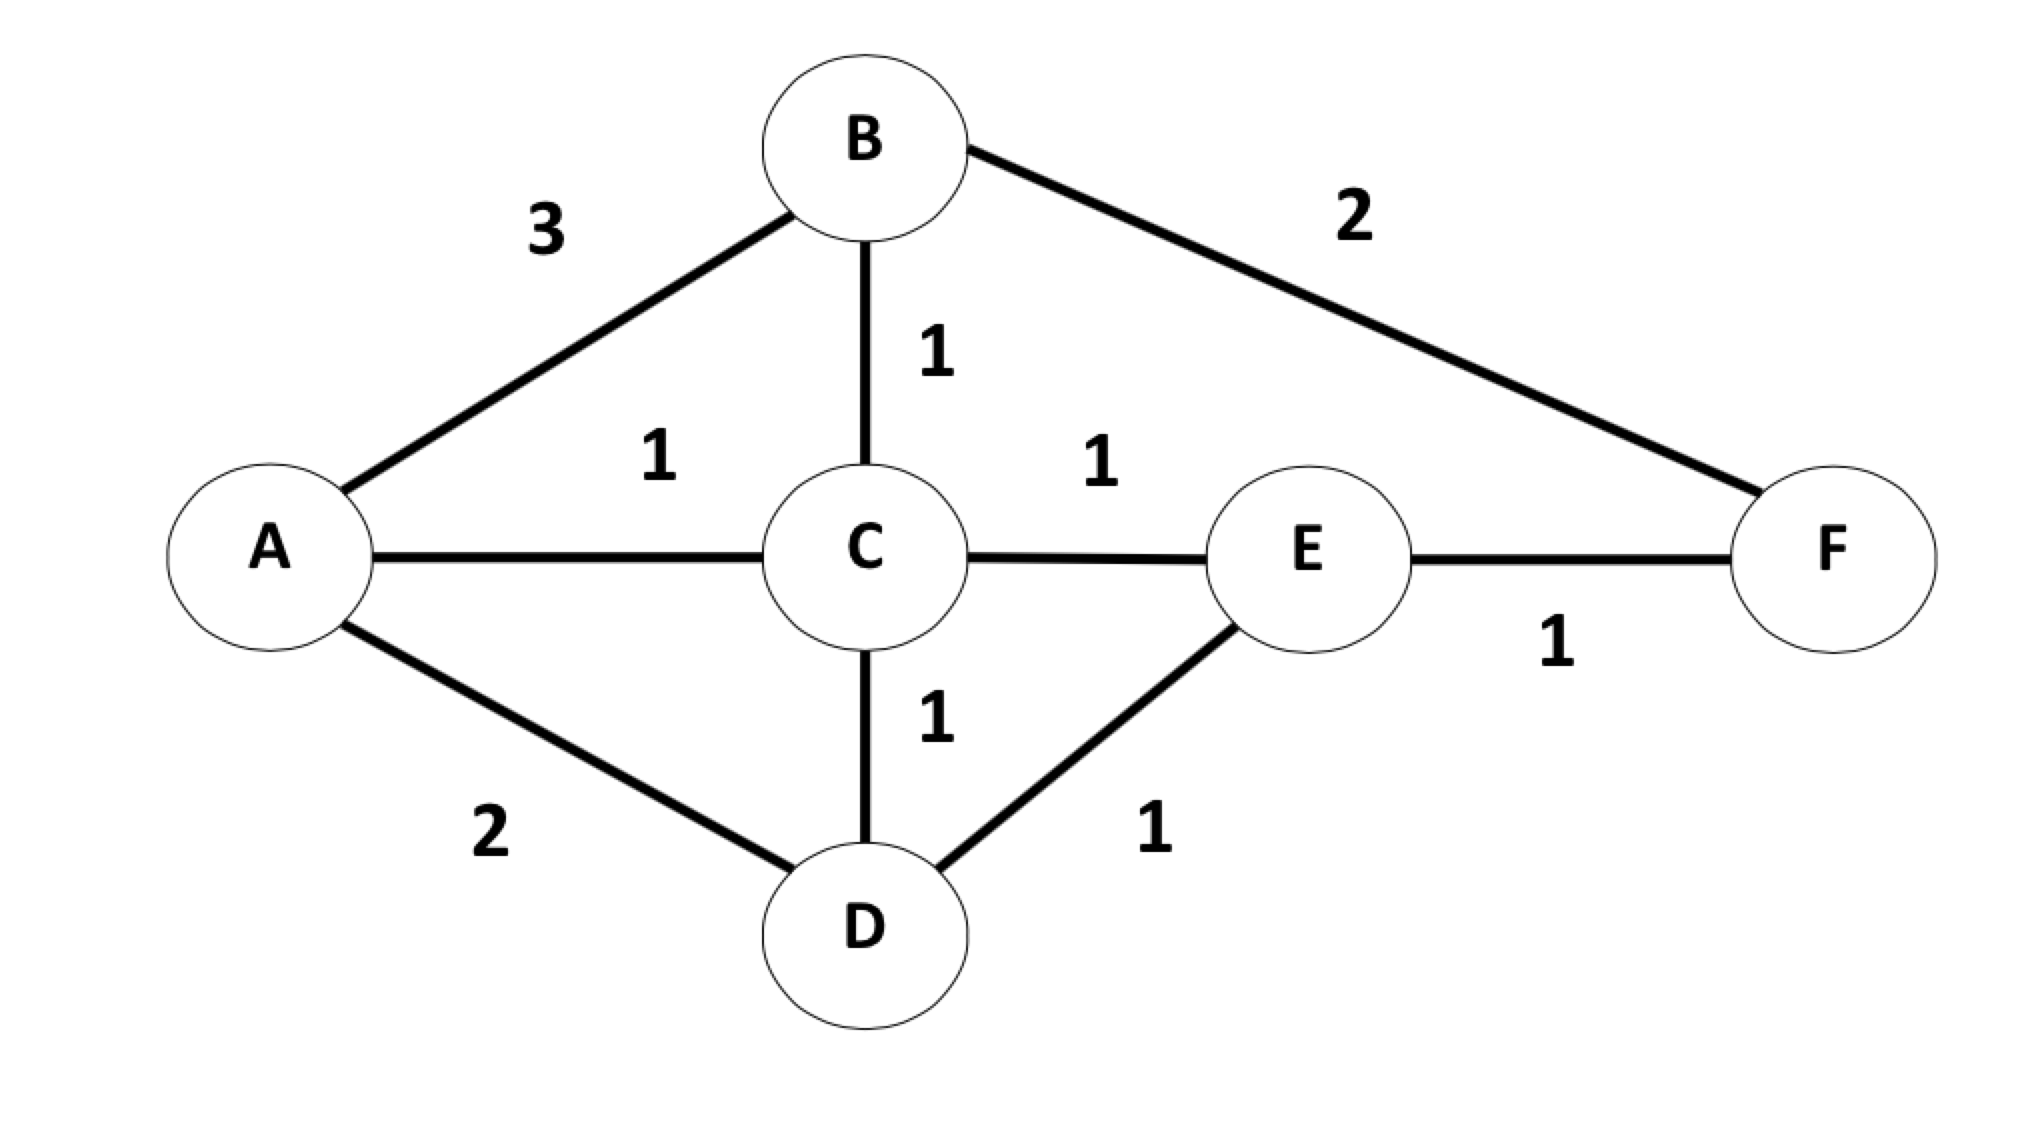
\includegraphics[width=0.75\textwidth]{16-figure-1}
            \end{figure}

            Now consider the network of Figure 1 and a Link-State Routing
            algorithm.

            \begin{subparts}
              \SetQuestionNumber{4}
              \subpart If $A$ sends a packet to $B$, what path does the packet
                take?

              \subpart If $A$ sends a packet to $F$, what path does the packet
                take?

              \subpart Now assume that the link cost for the links $C-E$ and
                $E-F$ both change to $6$. $E$ announces these changes and all
                nodes but $C$ get the update (that is, $C$ still thinks $C-E$
                and $E-F$ are link-cost $1$). Now $A$ sends to $F$, what path
                does the packet take?

              \subpart Finally, $C$ gets the new link-weight information and
                now knows that $C-E$ and $E-F$ are link-cost $6$. When $A$
                sends to $F$, what path does it take?

            \end{subparts}
        \end{parts}
      \question \textit{Supervision discussion questions}
        \begin{parts}
          \part Compare Forwarding versus Routing

          \part Compare and contrast Link-State Routing with Distance-Vector
            Routing. What are the (information) consistency models of each?
            What information is exchanged?

          \part What makes a fast LPM algorithm? (Longest-Prefix-Match)?

          \part What happens when (packet) fragment loss occurs?

          \part What is the state held by a NAT box? How does a NAT box work
            out its state?

          \part Why do packets tend towards the same path(route) through the
            network?

          \part How does ARP work?

          \part Compare DNS and ARP

          \part Why would I (or wouldn’t I) want to broadcast an ARP response?

          \part How does Gateway ARP do its thing?
        \end{parts}

      %%%%%%%%%%%%%%%%%%%%%%%%%%%%%%%
      \section*{Topic 05 - Transport}
      %%%%%%%%%%%%%%%%%%%%%%%%%%%%%%%

      \question \textit{Transport flavours}
        \begin{parts}
          \part The User Datagram Protocol (UDP) is sometimes used instead of
            TCP. It procides very few features above those provided by IP.

            \begin{subparts}
              \subpart Give one feature provided by UDP but not by IP, and one
                provided by UDP but not by TCP.

              \subpart Explain the role of a port number in UDP. Why isn’t it
                the Process ID? Explain the relation between TCP and UDP port
                numbers.

              \subpart Give three characteristics which might make an
                application protocol better suited to implementation over UDP
                than over TCP.

            \end{subparts}
        \end{parts}

      \question \textit{Error control, ARQ}
        \begin{parts}
          \part Why do error control protocols for packet switched networks use
            error detecting codes but not error correcting codes?

          \part A transport protocol for packet-switched networks uses a
            “sliding window” Automatic Repeat reQuest (ARQ) scheme for error
            control and flow control.

            \begin{subparts}
              \subpart As well as error detecting codes, ARQ protocols use
                acknowledgments and timeouts to achieve error control. Briefly
                explain what these are, and how they are combined to achieve
                reliable transmission.

              \subpart What two error cases might cause a receiver to send a
                negative acknowledgment (NACK)? How are they detected? What
                happens if the NACK is lost?

              \subpart In what circumstances will a receiver receive a packet
                with the same sequence number twice? What should it do in these
                circumstances?

              \subpart Given that the protocol provides bidirectional
                communication, what optimisation can be made in the
                implementation of acknowledgments to reduce the total number of
                packets sent?

              \subpart If two hosts are connected by a 100Mbps link with a
                round-trip time of 20ms, how big (in bytes) should the sliding
                window be to maximise link usage?

              \subpart Give two reasons why, at a given time, the window size
                might be set to a smaller value.

            \end{subparts}

          \part Consider a sliding window protocol with a window size of $5$
            using cumulative ACKs.

            \begin{description}
              \item[Retransmissions] retransmissions occur under two
                conditions: Reception of three duplicate ACKs (that is, three
                identical ACKs after the initial ACK) and Time out after
                100msec (timer starts at the beginning of the packet
                transmission)
              \item[Timing] Data packets have a transmission time of 1 msec.
                ACK packets have zero transmission time.
                The link has a latency of 10msec.
                The source A starts off by sending its first packet at time t=0.
            \end{description}

            \begin{subparts}
              \subpart Assume all packets are successfully delivered except the
                following:
                \begin{itemize}
                  \item The first transmission of data packet \#3
                  \item The ACK sent in response to the receipt of data packet
                    \#6
                \end{itemize}
                When is data packet \#3 first retransmitted (expressed in terms
                of msec after $t=0$)?

              \subpart Consider the same scenario, but with everything
                successfully delivered except the following:
                \begin{itemize}
                  \item The first transmission of data packet \#3
                  \item The first transmission of data packet \#5
                  \item The ACK sent in response to the receipt of data packet
                    \#6
                \end{itemize}

                When is data packet \#3 first retransmitted (expressed in terms
                of msec after $t=0$)?

              \subpart Assume we can only observe the ACK packets arriving at
                the sender.

                The same sliding window algorithm is used, with the same
                timings and retransmission policies apply.

                Notation (read carefully): The notation $Ax$ is used to mean
                that the ACK packet is acknowledging the receipt of all packets
                up to and including data packet $x$.

                That is, $A5$ is acknowledging the receipt of packet $5$; to be
                clear, the notation does not mean that the receiver is
                expecting packet $5$ as the next data packet.

                Assume that the following ACK packets arrive (just the ordering
                is shown, no timing information is provided):

                \begin{itemize}
                  \item $A1$
                  \item $A2$
                  \item $A3$
                  \item $A4$
                  \item $A5$
                  \item $A6$
                \end{itemize}

                Which of the following five scenarios (described only by the
                unusual events that occurred; assume all else functioned
                normally) would have produced such a series of ACKs? (consider
                all that apply)

                \begin{itemize}
                  \item Data packet number $4$ was dropped
                  \item Data packet number $4$ was delayed, arrived immediately
                    after data packet $5$
                  \item Data packet $3$ was duplicated by the network
                  \item ACK packet $A3$ was duplicated by the network
                  \item ACK packet $A4$ was delayed, arriving after $A5$
                \end{itemize}

              \subpart With the same set up as in the previous problem,
                consider the following stream of ACK packets.

                \begin{itemize}
                  \item $A1$
                  \item $A2$
                  \item $A3$
                  \item $A5$
                  \item $A4$
                  \item $A6$
                \end{itemize}

                Which of the following five scenarios (described only by the
                unusual events that occurred; assume all else functioned
                normally) would have produced such a series of ACKs? (consider
                all that apply)

                \begin{itemize}
                  \item Data packet number $4$ was dropped
                  \item Data packet number $4$ was delayed, arrived immediately
                  after data packet $5$
                  \item Data packet $3$ was duplicated by the network
                  \item ACK packet $A3$ was duplicated by the network
                  \item ACK packet $A4$ was delayed, arriving after $A5$
                \end{itemize}

              \subpart With the same set up as in the previous problem,
                consider the following stream of ACK packets.

                \begin{itemize}
                  \item $A1$
                  \item $A2$
                  \item $A3$
                  \item $A3$
                  \item $A5$
                  \item $A6$
                \end{itemize}

                Which of the following five scenarios (described only by the
                unusual events that occurred; assume all else functioned
                normally) would have produced such a series of ACKs? (consider
                all that apply)

                \begin{itemize}
                  \item Data packet number $4$ was dropped
                  \item Data packet number $4$ was delayed, arrived immediately
                  after data packet $5$
                  \item Data packet $3$ was duplicated by the network
                  \item ACK packet $A3$ was duplicated by the network
                  \item ACK packet $A4$ was delayed, arriving after $A5$
                \end{itemize}
            \end{subparts}
        \end{parts}

      \question \textit{TCP specifics}
        \begin{parts}
          \part Use the approcimate equation for throughput as a function of
            drop rate:

            $$ {throughput} = \frac{\sqrt{1.5}*{MSS}}{RTT\sqrt{p}}$$

            Assume an RTT of 40msec and an MSS of 1000 bytes. In the following
            questions ignore IP and TCP headers in your calculations

            \begin{subparts}
              \subpart What drop rate $p$ would lead to a throughput of 1Gbps?

              \subpart What drop rate $p$ would lead to a throughput of 10 Gbps?

              \subpart If the connection is sending data at a rate of 10Gbps,
                how long on average is the time interval between drops?

              \subpart What window size $W$ (measured in terms of MSSes) would
                be required to maintain a sending rate of 10Gbps? (rounded down
                to the nearest integer)

              \subpart If a connection suffered a drop upon reaching 10Gbps,
                how long would it take for it to return to 10Gbps (after
                undergoing a fast retransmit)? (in seconds, rounded down to the
                nearest second)

              \subpart Consider two TCP connections whose throughput obeys the
                TCP throughput equation listed above.

                The first TCP connection has the following parameters:
                ${MSS} = 1000 {bytes}$, ${RTT} = 0.2msec$, ${drop rate} = 0.5\%$

                The second TCP connection has the following parameters:
                $MSS = 2000 bytes$, $RTT = 0.1msec$, $drop rate = 8\%$

                What is the ratio of throughputs (the throughput of the first
                TCP connection divided by the throughput of the second TCP
                connection)? Why?

            \end{subparts}

          \part Consider the plot of CWND versus time for a TCP connection.
            \begin{subparts}
              \subpart At each of marked marked points along the timeline in
                the figure on the next page, indicate what event has happened,
                or what phase of congestion control TCP is in (as appropriate),
                from the following set: Slow-Start, Congestion-Avoidance,
                Fast-Retransmit, and Timeout.

              \subpart Assume CWND is 10,000 right before F, what is the value
                of SSTHRESH at G?

                %%%%%%%% GRAPH HERE
            \end{subparts}
        \end{parts}

      \question \textit{Supervision discussion questions}
        \begin{parts}
          \part What are four of the timers in the TCP ARQ?

          \part How do I recover from silly window syndrome?

          \part Why does UDP use port number and not process id?

          \part What is the effect of out-of-order delivery on Go-Back-N?

          \part What does congestion cause?

          \part Why does doubling the window-size cause exponential growth?

          \part How might duplicates occur in RDT 3.0?

          \part When/Why can you cache window-size information between
            connections?

          \part Why is reordering bad (for fast-transmit)?

          \part How does multiple routing paths screwup TCP?

        \end{parts}
    \end{questions}
\end{document}
